\section{Descripción del simulador} 
\label{xray:method}

La combinación del algoritmo propuesto en esta tesis, y la librería que permite simular rayos X permite crear un simulador para entrenar proyecciones radiológicas. En este simulador, el usuario podrá manipular cualquier variación de anatomía humana (ver sección \ref{posing:req}) y obtendrá de manera inmediata una imagen de rayos X simulada. En este sentido, el usuario podrá cargar cualquier modelo (previamente de ejecutar el proceso previo explicado en la sec. \ref{posing:preprocess}), configurar los parámetros del simulador de rayos X y obtener en tiempo real la imagen médica asociada. De esta manera, los usuarios pueden revisar multitud de escenarios, probar parámetros concretos, focalizarse en errores comunes que se realizan en los entornos reales o enfatizar pequeños detalles. Estudiantes y profesores pueden dedicar todo el tiempo necesario en una herramienta interactiva sin riesgo ninguno frente a la práctica en un entorno real. Además, pueden variar la anatomía  y parámetros que no es posible en los archivos educativos donde solo se encuentran imágenes estáticas. 

La integración de las dos herramientas ha resultado sencilla debido a que su funcionalidad no entra en conflicto con la otra. El proceso previo del algoritmo de posicionamiento se produce de la misma manera, y es en la fase de interacción (sec. \ref{posing:Poses}) donde las mallas superficiales se comparten entre las dos librerías. Gracias a las capacidades de  la arquitectura de las tarjetas gráficas, ambas librerías trabajan sobre el mismo conjunto de datos ya que comparten memoria en \ac{GPU}.

Los resultados visuales se presentan en una interfaz creada a propósito para permitir al usuario interaccionar con el simulador. Por una parte, podrá observar la representación 3D de las mallas superficiales cargadas y adicionalmente podrá observar la imagen de rayos X en todo momento, resultado de la proyección del emisor al detector. Esta proyección podrá ser modificada por el usuario a través del ratón o los botones diseñados para tal efecto. 

La figura \ref{fig:Posesummary} resumen la arquitectura final del simulador que partiendo con la anatomía de entrada, pasando por el proceso previo, los modelos son deformados y se consigue una imagen médica resultado de la configuración actual.

\begin{figure}[h]
\centering
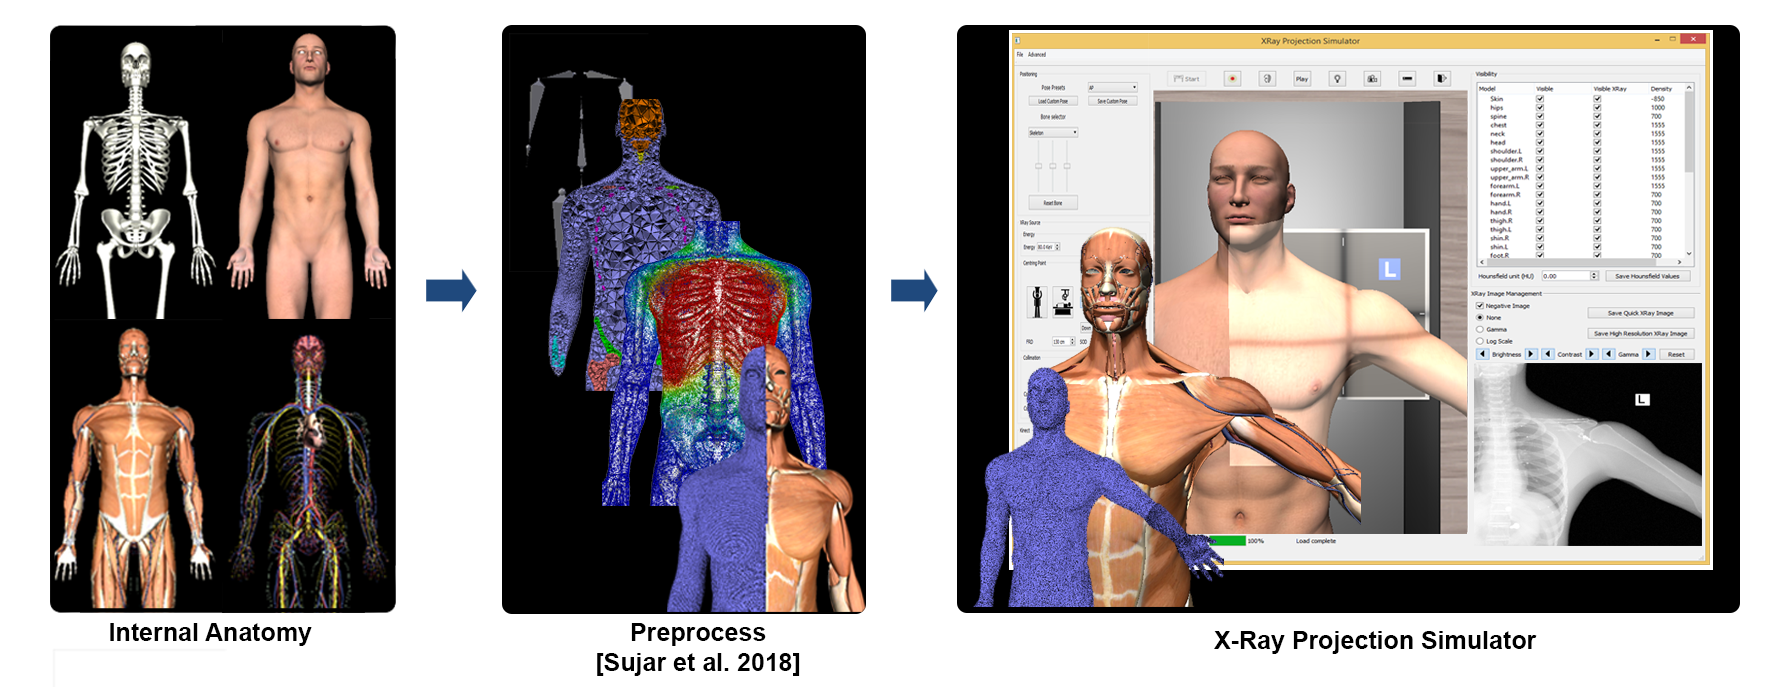
\includegraphics[width=\linewidth]{IMG/summary.png}

\caption{\label{fig:Posesummary} Arquitectura del simulador: i) modelos anatómicos de entrada ii) Proceso previo iii) Interfaz del simulador donde se ha integrado la \emph{selección de poses} con \emph{gVirtualXRay}.
}
\end{figure}

A continuación, se presentarán los casos de uso a los que se pretende atender con el simulador desarrollado.



\subsection{Caso de uso: Profesor}
\label{xray:casodeuso}
Los profesores imparten sus clases ayudados por presentaciones y siguen una lista de proyecciones radiológicas que quiere mostrar a los estudiantes. En el transcurso de la explicación de una proyección, el profesor puede cargar un modelo anatómico y enseñar interactivamente a realizar la proyección concreta.  Primero, el profesor explica la posición del paciente que debe tener para realizar la radiografía, moviendo las articulaciones que tenga el modelo disponible. A continuación explica cómo conseguir la configuración de la máquina de rayos X que permita conseguir la mejor imagen posible. El profesor puede centrarse en explicar cómo evitar los errores más comunes como una mala posición del centro de proyección, mala posición de marcadores de referencia, colimación pobre o una incorrecta configuración del emisor. Además, pueden realizar proyecciones incorrectas o posiciones incorrectas del paciente con la finalidad de que los estudiantes las identifiquen. Incluso, pueden simular enfermedades como la pancreatitis, piedras en el riñón o cuerpos extraños en la anatomía del paciente.


\subsection{Caso de uso: Estudiante}

Los estudiantes pueden usar esta herramienta como material adicional a sus libros y archivos de imágenes. Estos podrían revisar cada proyección explicada en el libro e intentar reproducirla en el simulador. Los estudiantes cargan un modelo anatómico y comienzan posicionando al paciente en su pose correcta. De pie, sentado, tumbado o mover cualquier articulación por separado si es necesario. Los estudiantes deberán configurar los parámetros del emisor de rayos X y centrar la proyección con forma de cruz proyectada por la luz del emisor, tal y como lo harían en un entorno real. Los estudiantes deben prestar atención a la colimación necesaria y poner el marcador de referencia en un sitio adecuado. La imagen médica resultante puede ser almacenada para ser utilizadas con otras intenciones.



\subsection{Casos de uso: Ejercicios de clase}

Los profesores pueden diseñar un ejercicio de clase en la herramienta. Se elaboran una lista con las proyecciones que se necesitan reforzar o evaluar y la herramienta les pedirá a los estudiantes realizarlas. Los estudiantes abren la aplicación que cargará el modelo anatómico automáticamente y se les solicitará que realicen una serie de proyecciones vistas en clase. Los estudiantes deberán realizar el procedimiento sin ver la imagen de rayos X intentando simular un entorno realista. Cuando el estudiante cree tener una buena proyección, puede obtener la imagen médica y el sistema le preguntará si está de acuerdo o quiere repetirla. Cuando el usuario considere que su proyección es correcta, la herramienta procederá con la siguiente y guardará un conjunto de métricas de evaluación junto con la imagen que serán evaluadas por el profesor. 


Por otra parte, el profesor puede realizar una serie de proyecciones y guardar las imágenes obtenidas. Estas imágenes serán presentadas a los estudiantes para que averigüen cual es la proyección que se intenta conseguir y los parámetros que deberían ser usados para conseguir una imagen similar.




\subsection{Posicionamiento del modelo anatómico}
\label{xray:posing}
En el diagnóstico por imagen la posición del paciente es esencial para poder obtener la mejor imagen médica reduciendo la cantidad de dosis recibida por el paciente y el tiempo empleado. La comodidad y la seguridad del paciente es fundamental y los radiólogos tienen que estar seguros de como colocar a un paciente para evitar repeticiones y exposiciones adicionales a los rayos X. En esta herramienta, gracias al algoritmo propuesto de posicionamiento, el usuario es capaz de modificar la postura del modelo anatómico cargado con el objetivo de aprender a conseguir una pose correcta. Los usuarios pueden interaccionar con las articulaciones disponibles del modelo virtual. En la figura \ref{fig:pose}, el brazo ha sido posicionado con el objetivo de conseguir una proyección del codo. Se pueden crear posiciones predefinidas por los profesores para que los estudiantes puedan usarlas en el futuro.



\begin{figure}[h]
\centering
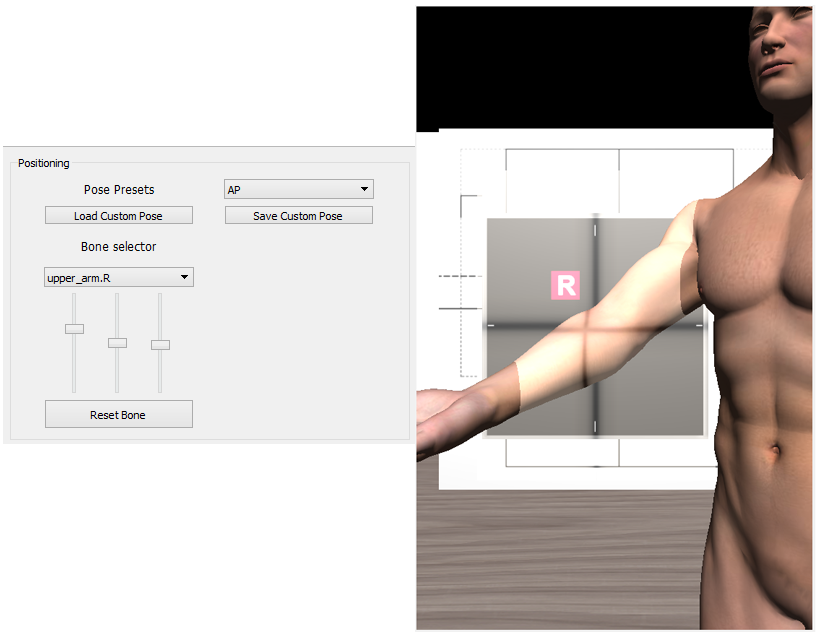
\includegraphics[width=0.5\linewidth]{IMG/Pose.png}
\caption{\label{fig:pose}Ejemplo de proyección de codo }
\end{figure}

Aunque no haya consecuencias físicas en las imágenes si el paciente se encuentra de pie o tumbado, este aspecto es relevante médicamente y es importante en el currículum de los estudiantes. El usuario puede cambiar de postura en cualquier momento con los botones que se pueden observar en la figura \ref{fig:setup}.




\subsection{Configuración del emisor de rayos X}
\label{xray:setupxray}

Los factores de exposición es un aspecto fundamental en el diagnóstico por imagen ya que afecta tanto a la seguridad del paciente como a la calidad de la imagen de radiografía. Una configuración inapropiada del emisor puede producir un mal contraste en la imagen, siendo el objetivo final prevenir repeticiones innecesarias. Los estudiantes deben tener en cuenta que la radiación de los rayos X es absorbida de forma diferente entre los tejidos blandos y densos. Por otra parte, la configuración de la \ac{kvp} o kilovoltaje es un factor influyente en la exposición radiográfica, ya que afecta la calidad del haz. El aumento de \ac{kvp} produce rayos más penetrantes consiguiendo más exposición en la imagen. Si es demasiado alto, resultará en sobre exposición y la imagen resultante será muy oscura. Si es demasiado bajo, la imagen quedará más desenfocada y blanquecina.

En la figura \ref{fig:setup}, se puede observar la diferencia entre dos configuraciones del emisor diferentes. El usuario puede jugar con los parámetros que le ayudarán a entender como los cambios en el \ac{kvp} afectan a la imagen de manera inmediata. 




\begin{figure}[tb]
\centering
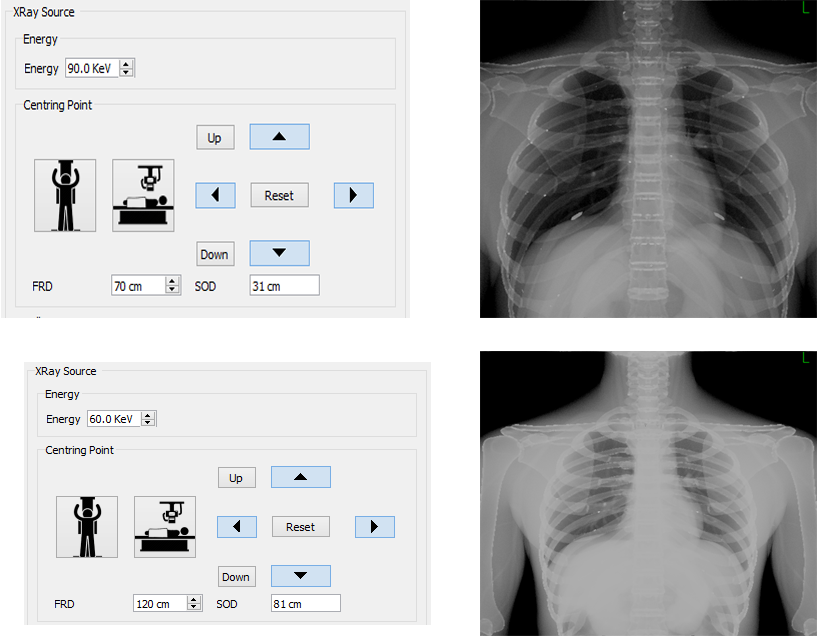
\includegraphics[width=0.5\linewidth]{IMG/setup.png}
\caption{\label{fig:setup} Ejemplos distintos de configuración del emisor. Arriba podemos observar sobre exposición y una imagen más oscura. Por otro lado, abajo hay poca exposición que resulta en una imagen borrosa y blanquecina. }
\end{figure}

\subsection{Centro de proyección y colimación}

Posicionar correctamente el centro de la proyección y la colocación del paciente es fundamental para reducir la cantidad de radiación que recibe el paciente. El radiólogo siempre tiene que asegurarse que la zona objetivo del cuerpo en el centro de la proyección y del panel del detector. La colimación es la técnica de limitar la proyección del haz saliente del emisor con unas placas de plomo. Esta técnica es importante para limitar el área objetivo de la anatomía, mitigar la radiación que recibe el paciente, reducir la dispersión de la radiación y mejorar la calidad de la imagen.  

Todos estos parámetros han sido introducidos en el simulador, donde los estudiantes o profesores pueden practicar estos conceptos. A través de la interfaz 3D los usuarios pueden mover con el ratón la luz proyectada desde el emisor (ver Fig. \ref{fig:collimation}) o pueden usar los botones de la interfaz para conseguir una buena colocación de la proyección (ver Fig. \ref{fig:setup}).


\begin{figure}[tb]
\centering
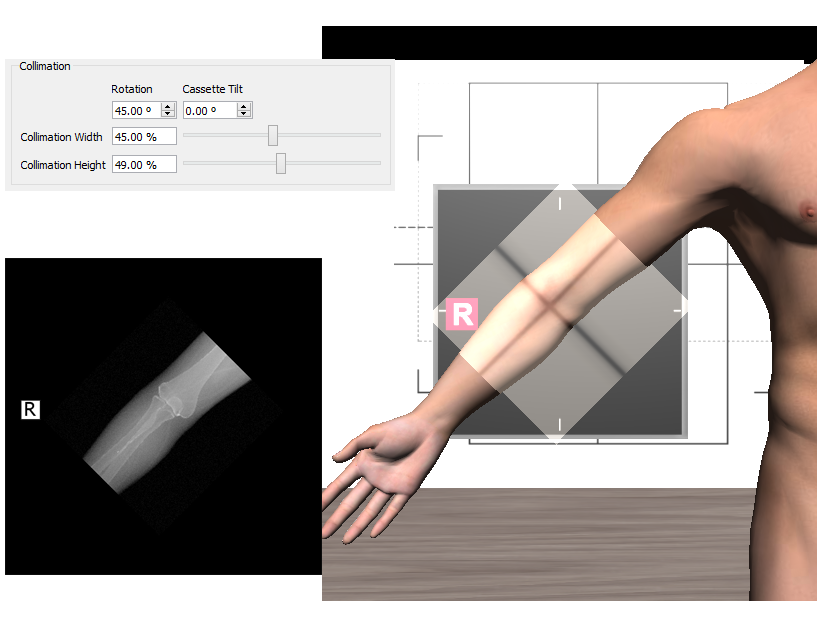
\includegraphics[width=0.5\linewidth]{IMG/collimation.png}
\caption{\label{fig:collimation} Colimación rotada a 45º para conseguir una imagen colimada del codo.}
\end{figure}


\subsection{Marcas de referencia}
\label{xray:sidemark}
Una buena práctica en radiología es colocar una marca de referencia que será visible en la imagen médica. Estos marcadores se utilizan para identificar qué lado del paciente está siendo capturado, con el objetivo de reducir errores y repeticiones. Esta práctica es prácticamente obligatoria debido a evitar que otros médicos puedan errar en la interpretación de la imagen. En el simulador se ha incorporado la funcionalidad para que el usuario pueda posicionar el marcador interactivamente con el ratón. Este marcador será inmediatamente incorporado en la textura del panel que se puede ver en la interfaz 3D y será visible también en las imágenes guardadas. En la figura \ref{fig:side} se puede observar la división de la interfaz donde el usuario puede interaccionar y el resultado en la escena 3D. 



\begin{figure}[h]
\centering
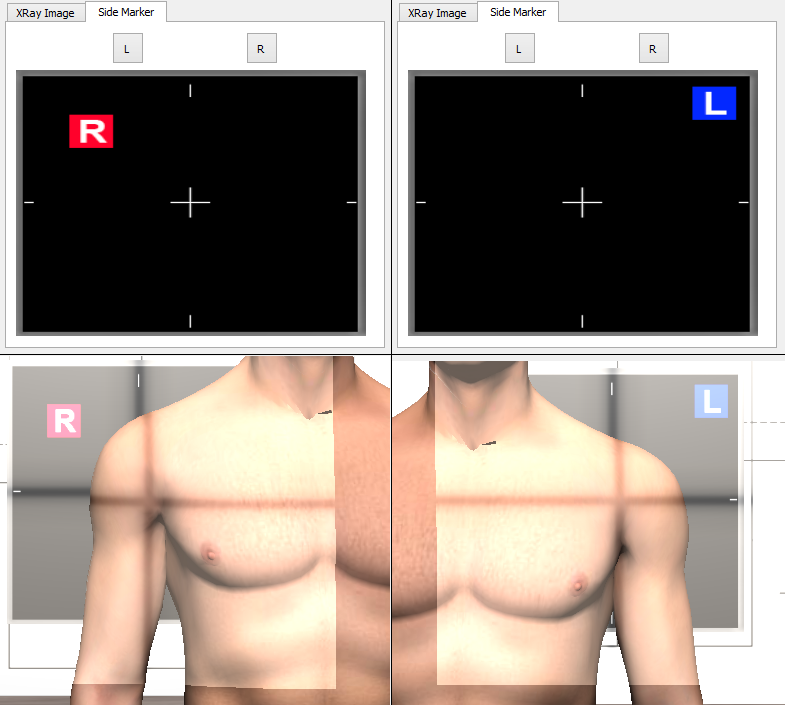
\includegraphics[width=0.5\linewidth]{IMG/side.png}
\caption{\label{fig:side} Se puede seleccionar el marcador izquierda o derecha y situarlo en el panel.}
\end{figure}


\subsection{Variedad de casos}
\label{xray:variedad}
Una de las ventajas que presenta este simulador frente a los archivos de imágenes y libros es la posibilidad de modificar la anatomía del paciente. Los usuarios puede ocultar ciertos tejidos en la ventana donde se muestra la escena 3D. De esta manera, el usuario podrá entender donde se sitúan o como se mueven los tejidos que se encuentran dentro de la piel. Incluso, es posible ocultar objetos tanto visualmente como al simulador de rayos X para ver las imágenes resultantes con la ausencia de estos tejidos. 

Otra ventaja que el simulador proporciona es la posibilidad de modificar la anatomía interna y sus propiedades físicas con el objetivo de conseguir más variabilidad. Los usuarios pueden modificar la escala de \emph{Hounsfield} o su composición química para conseguir mostrar el efecto de ciertas enfermedades y su imagen radiológica asociada. Por ejemplo, un usuario puede calcificar un hueso, representar un pulmón colapsado o ilustrar un estómago lleno de aire como se puede ver en la figura \ref{fig:disease}. Es incluso posible, añadir objetos extraños dentro de la anatomía del paciente y permitir al usuario identificarlas desde infinidad de puntos de vista.

\begin{figure}[h]
\centering
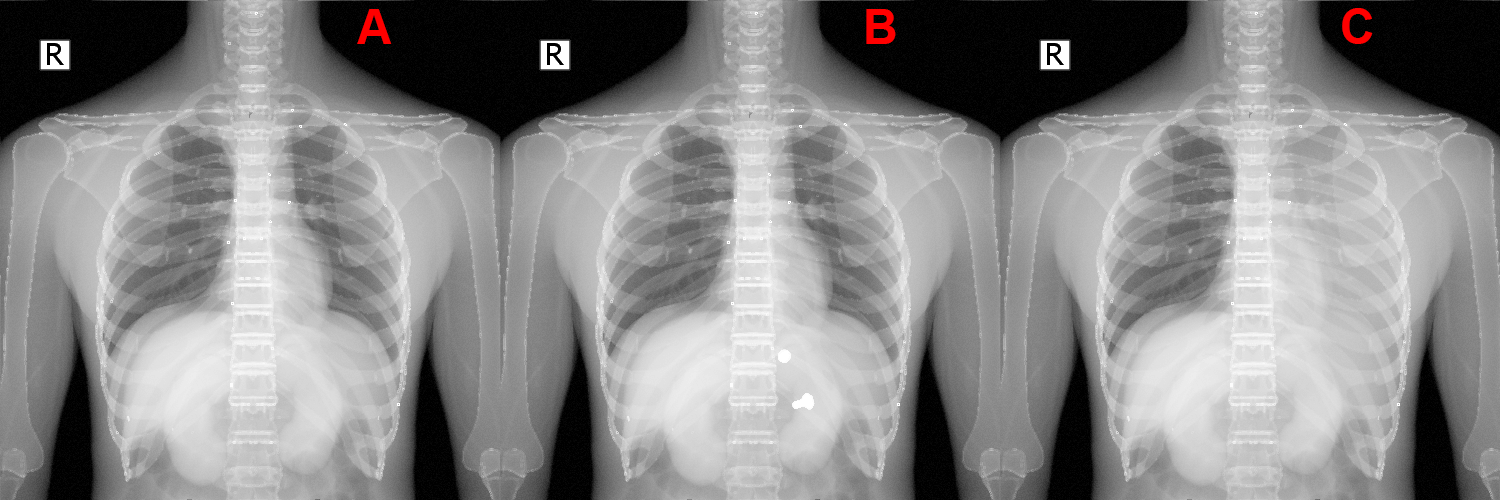
\includegraphics[width=0.5\linewidth]{IMG/disease.png}
\caption{\label{fig:disease} Los usuarios pueden simular variedad de casos. A: Aspecto normal. B: Objetos extraños en el estómago. C: Pulmón izquierdo colapsado }
\end{figure}

\subsection{Ajuste de la imagen}
\label{xray:ajustes}
En la sección \ref{xray:setupxray}, el usuario puede configurar y familiarizarse con el concepto de \ac{kvp} con el objetivo de mejorar la imagen radiológica. Aun así, actualmente existen detectores digitales en los hospitales modernos que permiten capturar la imagen médica de forma digital. Esta imagen digital se podrá mostrar en un ordenador instantáneamente. Quizás en el futuro, se podrá utilizar diagnósticos asistidos por computador, pero en la actualidad es necesario la intervención humana para interpretar las imágenes resultantes. La ventaja de la imagen digital es la posibilidad de duplicar, almacenar y manipular la imagen médica. Esto permite a los usuarios a manipular la imagen capturada con el objetivo de reducir los errores de sobre-exposición o sub-exposición producido por una mala configuración del emisor. Incluso, se puede conseguir más información de la imagen a través de programas de edición de imágenes que permiten observar detalles mínimos que no puede verse a simple vista.  

Los usuarios, como pudieran hacerse en la realidad, pueden manipular la imagen obtenida con algunas funcionalidades implementadas en el simulador. Se puede cambiar el brillo y el contraste para enfatizar o remarcar las diferencias entre tejidos. Por otro lado, se han implementado un filtro gamma y un filtro logarítmico con el objetivo de mejorar la imagen capturada. El usuario puede modificar estos parámetros con el ratón y los botones integrados en la interfaz. En la figura \ref{fig:imgmani} muestra un ejemplo de manipulación de la imagen capturada con la misma configuración del emisor de rayos X.
Finalmente, las imágenes manipuladas se pueden guardar en el disco duro.


\begin{figure}[h]
\centering
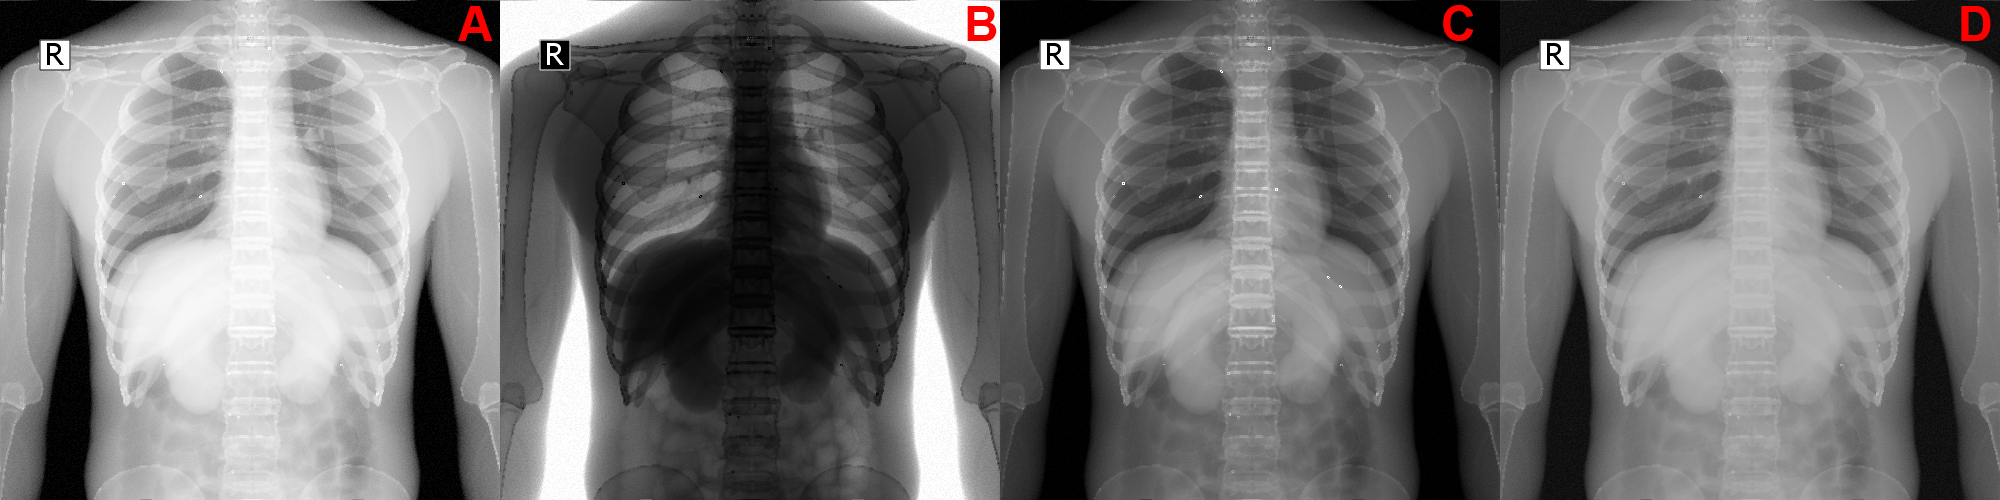
\includegraphics[width=0.5\linewidth]{IMG/imgmanipulation.png}
\caption{\label{fig:imgmani} A: Imagen de referencia. B: Imagen en negativo. C: Imagen utilizando filtro Gamma. D: Imagen con filtro logarítmico. }
\end{figure}

\todo{Añado lo de meter ruido en la imagen?}

\subsection{Simulador como herramienta de aprendizaje}
\label{xray:sim}
Con el objetivo de obtener buenas competencias para realizar proyecciones radiológicas, los estudiantes pueden practicar la teoría en el simulador y mejorar su confianza en el procedimiento. En este contexto, los simuladores de \ac{RV} proporcionan el entorno seguro para enseñar o practicar procedimientos peligrosos para el paciente, pero es necesario una aplicación diseñada para guiar y mejorar el proceso de aprendizaje de los estudiantes. El simulador se ha diseñado para que se pueda utilizar de dos formas. 
Orientado al estudiante, se ha diseñado un modo guiado que dirige al usuario durante el procedimiento y las funcionalidades del simulador. Este modo puede explicar cómo conseguir una buena proyección radiológica y ofrecer ayuda adicional al usuario si lo requiere.

Otro modo es utilizarlo como método de evaluación. Los estudiantes pueden realizar un ejercicio realizado por sus profesores previamente. Los estudiantes son requeridos de realizar proyecciones concretas sin poder visualizar la imagen radiológica inmediatamente. El estudiante debe posicionar al paciente y configurar el emisor de rayos X al igual que haría en un entorno real. De esta forma, cuando estén seguros de su colocación, estos podrán tomar la radiografía. Los profesores pueden permitir repeticiones o no además de que el simulador guardará métricas de evaluación y las imágenes resultantes para que el profesor pueda evaluar al estudiante su desempeño.

Antes de utilizar el simulador, el usuario puede revisar material multimedia que ayuda a familiarizarse con los elementos del simulador.

